% (C) 2020 Diogo Rodrigues
% Licensed under Creative Commons Attribution-NonCommercial-NoDerivatives 4.0 International (CC-BY-NC-ND 4.0)

\documentclass{bdad}
\usepackage[english]{babel}
% Metadata
\title{SOPE -- Test 2020}
\author{Diogo Miguel Ferreira Rodrigues \\ \href{mailto:dmfrodrigues2000@gmail.com}{dmfrodrigues2000@gmail.com}}
% Document
\begin{document}

\renewcommand{\theenumi}{\alph{enumi}}

\exam{Test 2020}

\question{Question 1}
Select the correct answer(s) about the given diagram:

\begin{center}
    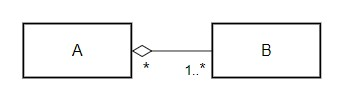
\includegraphics[scale=0.8]{2020T-01.jpg}
\end{center}

\begin{enumerate}
    \item \checkbox~B is part of A
    \item \checkbox~If an instance of A is deleted, the instances of B it contains are also deleted
    \item \checkbox~An instance of B can exist without the existence of any instance of A
    \item \checkbox~The same instance of B can only be part of one instance of A
\end{enumerate}

\question{Question 2}
In an UML class diagram, atomic attributes are those which:

\begin{enumerate}
    \item Are part of a key
    \item Have a domain containing only atomic values and the attribute contains only a single value from that domain
    \item Can be determined from other attribute(s)
    \item Can identify an object uniquely
    \item I don't want to answer
\end{enumerate}

\newpage
\question{Question 3}
Consider the conceptual model of a hospital's database, where information on patients admitted with COVID-19 is stored. It is intended to change the model, represented below, to make it possible to store the evolution of the patients' situation regarding the infection (infected, recovered, reinfected). What is the best way to proceed?

\begin{center}
    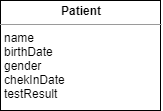
\includegraphics[scale=0.8]{2020T-03.png}
\end{center}

\begin{enumerate}
    \item I don't want to answer
    \item 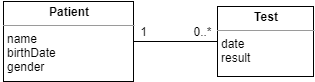
\includegraphics[scale=0.8]{2020T-03b.png}
    \item 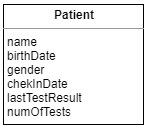
\includegraphics[scale=0.8]{2020T-03c.png}
    \item 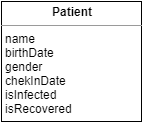
\includegraphics[scale=0.8]{2020T-03d.png}
    \item 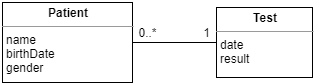
\includegraphics[scale=0.8]{2020T-03e.png}
\end{enumerate}

\question{Question 4}
When should we use a generalization?

\begin{enumerate}
    \item When subclass is the part and the superclass is the whole
    \item When subclass is a member of superclass
    \item I don't want to answer
    \item When both super and subclass have attributes in common
    \item When subclass is the whole and the superclass is the part
\end{enumerate}

\question{Question 5}
In UML class diagram, how does a derived attribute affect redundancy?

\begin{enumerate}
    \item Stored derived attributes are always redundant
    \item Stored derived attributes are not redundant
    \item Due to the high possibility of gaining additional knowledge from a derived attribute, they are always redundant
    \item Since you store the derived attribute and all data necessary to derive it, derived attributes cannot affect redundancy.
    \item I don't want to answer
\end{enumerate}

\question{Question 6}
When we want to convert many-to-one associations to the relational model by adding an additional relation with a key from the many side, what advantages will it bring to the schema?

\begin{enumerate}
    \item \checkbox~Increased rigour of the schema
    \item \checkbox~Increased performance due to a larger number of relations
    \item \checkbox~Increased performance due to a smaller number of relations
    \item \checkbox~Increased extensibility
\end{enumerate}

\newpage
\question{Question 7}
Consider the following UML diagram and its conversion to the relational model. Which are the two most adequate conversions?

\begin{center}
    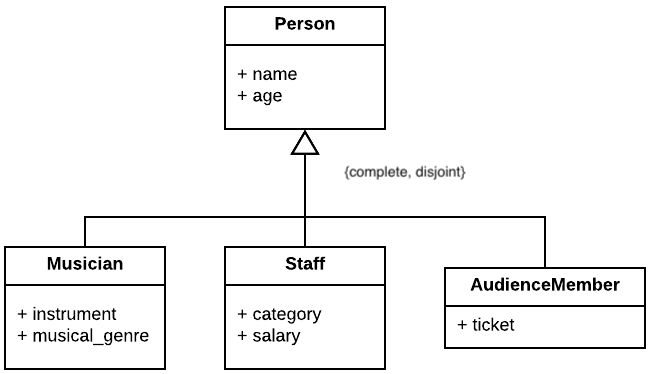
\includegraphics[scale=0.3]{2020T-07.png}
\end{center}

\begin{enumerate}
    \item \checkbox
\begin{blocklisting}
Person(id, name, age, instrument, musical_genre, category, salary, ticket)
\end{blocklisting}
    \item \checkbox
\begin{blocklisting}
Musician(name, instrument, musical_genre)
Staff(name, category, salary
AudienceMember(name, ticket)
\end{blocklisting}
    \item \checkbox
\begin{blocklisting}
Musician(id, name, age, instrument, musical_genre)
Staff(id, name, age, category, salary)
AudienceMember(id, name, age, ticket)
\end{blocklisting}
    \item \checkbox
\begin{blocklisting}
Person(id, name, age)
Musician(id->Person, name, instrument, musical_genre)
Staff(id->Person, name, category, salary)
AudienceMember(id->Person, name, ticket)
\end{blocklisting}
\end{enumerate}

\newpage
\question{Question 8}
Consider the following conceptual model. Mapping it to the relational model

\begin{center}
    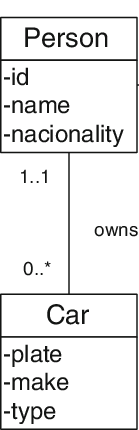
\includegraphics[scale=0.8]{2020T-08.png}
\end{center}

\begin{enumerate}
    \item \checkbox~Can result in 3 relations, one of them with a compound primary key
    \item \checkbox~Can result in 3 relations, two of them without foreign keys
    \item \checkbox~Can result in 2 relations with a foreign key in Car
    \item \checkbox~Can result in 2 relations with a foreign key in Person
\end{enumerate}

\question{Question 9}
There are three main methods that convert an UML into a Relation regarding Generalizations. Which one(s) is/are commonly used for overlapping generalizations?

\begin{enumerate}
    \item \checkbox~Use of NULLs
    \item \checkbox~Object-oriented
    \item \checkbox~E/R style
\end{enumerate}

\question{Question 10}
Mapping a ternary association and its associated classes

\begin{enumerate}
    \item \checkbox~Is affected by the number of associated classes
    \item \checkbox~Is affected by the multiplicity
    \item \checkbox~Can be converted to 3 relations
    \item \checkbox~Always results in 4 relations
\end{enumerate}

\question{Question 11}
A table in Boyce Codd Normal Form:

\begin{enumerate}
    \item \checkbox~Can have redundancy in some cases.
    \item \checkbox~Cannot assure dependency preservation.
    \item \checkbox~Cannot be subject of deletion anomalies.
    \item \checkbox~May be subject of update anomalies.
\end{enumerate}

\question{Question 12}
Consider the relation $R (A, B, C, D, E, F, G, H, I)$ with the following functional dependencies:

\begin{alignat*}{2}
    & A    && \rightarrow D \\
    & B    && \rightarrow I \\
    & B, D && \rightarrow H \\
    & A, E && \rightarrow C \\
    & F, G && \rightarrow E 
\end{alignat*}

Which attributes belong to the closure of $\{A, F, G\}$?

\begin{enumerate}
    \item \checkbox~$A$
    \item \checkbox~$B$
    \item \checkbox~$C$
    \item \checkbox~$D$
    \item \checkbox~$E$
    \item \checkbox~$F$
    \item \checkbox~$G$
    \item \checkbox~$H$
    \item \checkbox~$I$
\end{enumerate}

\question{Question 13}
Regarding decompositions, identify the correct statements.

\begin{enumerate}
    \item \checkbox~If $R_1$ and $R_2$ are a decomposition of $R$, the functional dependencies of $R$ are preserved in $R_1$ and $R_2$
    \item \checkbox~If we decompose to BCNF, the final schema will also be in 3NF
    \item \checkbox~If $R_1 \naturaljoin R_2=R$, $R_1$ and $R_2$ make a decomposition of $R$
    \item \checkbox~If $R_1$ and $R_2$ are a decomposition of $R$, the functional dependencies of $R$ are always preserved in $R_1$ or $R_2$
\end{enumerate}

\newpage
\question{Question 14}
Consider the relation $R (A, B, C, D, E, F, G, H, I)$ with the following functional dependencies:

\begin{alignat*}{2}
    & A    && \rightarrow D \\
    & B    && \rightarrow I \\
    & B, D && \rightarrow H \\
    & A, E && \rightarrow C \\
    & F, G && \rightarrow E
\end{alignat*}

What are the functional dependencies of the relation $S (A, B, H)$, a projection of $R$ in 3 attributes?

\begin{enumerate}
    \item $S$ has the same functional dependencies as $R$
    \item I don't want to answer.
    \item $A, B \rightarrow H$
    \item $A\rightarrow D$; $B\rightarrow I$; $A, B \rightarrow  D, H, I$; $A, H\rightarrow D$; $B, H\rightarrow I$
    \item $A\rightarrow D$; $B\rightarrow I$; $B, D\rightarrow  H$; $A, E\rightarrow C$
\end{enumerate}

\question{Question 15}
What is a minimal superkey?

\begin{enumerate}
    \item \checkbox~Primary key
    \item \checkbox~Foreign key
    \item \checkbox~Secondary key
    \item \checkbox~Candidate key
\end{enumerate}

\question{Question 16}
Consider you select a single numeric attribute as the primary key of a table. What is the most suitable data type for the primary key column in SQLite?

\begin{enumerate}
    \item \texttt{INTEGER} or \texttt{REAL} depending on the characteristics of the value.
    \item \texttt{REAL} if a big range of values is needed and \texttt{INTEGER} otherwise.
    \item \texttt{INTEGER} if autoincrement is needed and \texttt{REAL} otherwise.
    \item I don't want to answer.
    \item \texttt{INTEGER} because SQLite will automatically create an implicit column called rowid.
\end{enumerate}

\newpage
\question{Question 17}
We wish to add a foreign key to the table \texttt{T} that references table \texttt{A} (the primary key of \texttt{A} is an \texttt{int} called \texttt{AID}).

We also wish to update the foreign key when the primary key of \texttt{A} is updated.

\begin{enumerate}
    \item
    \begin{lstlisting}[language=SQL, numbers=none, frame=none, belowskip=0pt]
MODIFY TABLE T ADD AID int REFERENCES A(AID) ON UPDATE PROPAGATE;
    \end{lstlisting}

    \item
    \begin{lstlisting}[language=SQL, numbers=none, frame=none, belowskip=0pt]
MODIFY TABLE T ADD AID int REFERENCES A(AID) ON UPDATE CASCADE;
    \end{lstlisting}

    \item I don't want to answer

    \item
    \begin{lstlisting}[language=SQL, numbers=none, frame=none, belowskip=0pt]
ALTER TABLE T ADD AID int REFERENCES A(AID) ON UPDATE PROPAGATE;
    \end{lstlisting}

    \item
    \begin{lstlisting}[language=SQL, numbers=none, frame=none, belowskip=0pt]
ALTER TABLE T ADD AID int REFERENCES A(AID) ON UPDATE CASCADE;
    \end{lstlisting}
\end{enumerate}

\question{Question 18}
Analyse the following SQL script:

\begin{lstlisting}[language=SQL]
pragma foreign_keys=ON;
drop table if exists Product;
drop table if exists Package;
create table Product (id integer, price real);
create table Package (id integer, idProd integer, amount integer);
\end{lstlisting}

Assume you are asked to modify the script so that the attribute "idProd" is a foreign key that corresponds to the "id" attribute in the Product relation. Additionally, the "idProd" attribute should never have a NULL value and when its value is updated we want the "cascade" behaviour to be used. A database engineer was given this task and came up with the answers shown below (assume the rest of the script remains identical to the one shown above). Which of the answers is correct?

\begin{enumerate}
    \item I don't want to answer

    \item 
\begin{lstlisting}[language=SQL, numbers=none, frame=none, belowskip=0pt]
CREATE TABLE Package (
    id INTEGER,
    idProd INTEGER REFERENCES Product ON UPDATE CASCADE NOT NULL,
    amount INTEGER
);
\end{lstlisting}

    \item 
\begin{lstlisting}[language=SQL, numbers=none, frame=none, belowskip=0pt]
CREATE TABLE Package (
    id integer PRIMARY KEY, 
    idProd INTEGER REFERENCES Product(id) on UPDATE CASCADE NOT NULL, 
    amount INTEGER
);
\end{lstlisting}

    \item 
\begin{lstlisting}[language=SQL, numbers=none, frame=none, belowskip=0pt]
CREATE TABLE Package (
    id INTEGER, 
    idProd INTEGER REFERENCES Product NOT NULL ON UPDATE CASCADE, 
    amount INTEGER
);
\end{lstlisting}

    \item 
\begin{lstlisting}[language=SQL, numbers=none, frame=none, belowskip=0pt]
CREATE TABLE Package (
    id INTEGER PRIMARY KEY, 
    idProd INTEGER REFERENCES Product NOT NULL ON UPDATE CASCADE, 
    amount INTEGER
);
\end{lstlisting}
\end{enumerate}

\question{Question 19}
Which statement is wrong about the PRIMARY KEY constraint in SQL?

\begin{enumerate}
    \item Primary key can be made of multiple attributes
    \item A PRIMARY KEY uniquely identifies each record in a table
    \item Primary keys must contain UNIQUE values
    \item Primary key can be made of any single attributes
    \item I don't want to answer
\end{enumerate}

\question{Question 20}

A video streaming service has its database related to films and actors. A film consists of one or more actors. Each film has an identification number, a title and a duration. Each actor has a name and a nationality. Each actor is present at least in one film inserted in the database. The role of the actor in the film is classified by a name and a description. Both film and an actor may have received one or more awards. An award is determined by its name and description.

Considering the following sentences:

\begin{enumerate}[label=\Roman* - ]
    \item Film, actor and award are classes
    \item The multiplicity between film and actor is many to many 
    \item Role is a attribute
\end{enumerate}

Which ones are correct given the video streaming problem?

\begin{enumerate}
    \item I don't want to answer.
    \item I and II
    \item II and III
    \item Only I
    \item I, II and III
\end{enumerate}

\question{Question 21}
Consider the following relations:

\begin{center}
    \begin{tabular}{c c c}
        Car & Color & Interior \\
        \begin{tabular}{l | l}
            \textbf{carmodel}  	& \textbf{price} \\ \hline
            320 	    & 15000 \\
            340 	    & 17500 \\
            420 	    & 25000
        \end{tabular} &
        \begin{tabular}{l}
            \textbf{color} \\ \hline
            White \\
            Black \\
            Blue
        \end{tabular} &
        \begin{tabular}{l}
            \textbf{interiortype} \\ \hline
            Leather \\
            Nylon \\
            Polyester
        \end{tabular}
    \end{tabular}
\end{center}
In this system, Cars can be sold with all available interior colors, interior materials and outside paint.

Which of the following queries represents all possible combinations of cars, with varying interior types, interior colors and outside paint, but the colors of the interior and the car are different? 

\begin{enumerate}
    \item $\sigma_{Interior.color <> Car.color} (Car \times Color \times Interior \times (\rho_{interiorColor(color)} Color))$
    \item $Car \times Color \times Interior \times (\rho_{interiorColor(color)} Color))$
    \item $\sigma_{interiorcolor <> color} (Car \times Color \times Interior \times (\rho_{interiorColor(color)} Color))$
    \item $\sigma_{Interior.color <> Car.color} (Car \times Color \times Interior \times Color)$
    \item I do not wish to answer
\end{enumerate}

\question{Question 22}
What's the equivalent of the following SQL query in Relational Algebra:

\begin{lstlisting}[language=SQL, numbers=none, frame=none, belowskip=0pt]
SELECT a,b FROM T1 NATURAL JOIN (SELECT * FROM T2 WHERE c='John');
\end{lstlisting}

\begin{enumerate}
    \item $\pi_{a,b} (T1 \naturaljoin \sigma_{c='John'} (T2))$
    \item $\pi_{c='John'} (T1 \naturaljoin \sigma_{a,b} (T2))$
    \item $\sigma_{a,b} (T1 \naturaljoin \pi_{c='John'} (T2))$
    \item I do not wish to answer
    \item $\sigma_{a,b,c} (T1 \naturaljoin T2)$
\end{enumerate}

\question{Question 23}
If two relations $R$ and $S$ are joined, then the non-matching tuples of both $R$ and $S$ are ignored in which type of join?

\begin{enumerate}
    \item Right Inner Join
    \item Full Outer Join
    \item Inner Join
    \item Left Outer Join
    \item I do not wish to answer
\end{enumerate}

\question{Question 24}
Given $R(A, B, C, D)$, $S(A, C, E)$, what is the schema of $R \naturaljoin S$?

\begin{enumerate}
    \item $(A, C, B, D, E)$
    \item I do not wish to answer
    \item $(A, B, C, D)$
    \item $(B, D, E)$
    \item $(A, C, E)$
\end{enumerate}

\newpage
\question{Question 25}
\begin{center}
    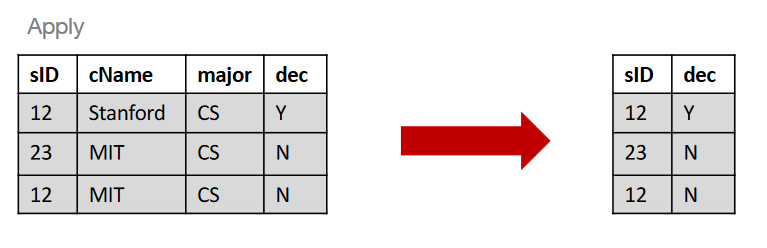
\includegraphics[scale=0.4]{2020T-25.png}
\end{center}

\begin{enumerate}
    \item $\sigma_{(sID = '12'~\vee~sID = '23')} Apply$
    \item $\pi_{(sID,dec)} Apply$
    \item I do not wish to answer
    \item $\pi_{(sID,dec)} (\sigma_{(sID = '12')} Apply)$
    \item $\sigma_{(dec = 'Y'~\vee~dec = 'N')} Apply$
\end{enumerate}

\end{document}